% MedVisionQuery — revised final report (October 2026).
% Build: tectonic main.tex   (or pdflatex main.tex twice)
\documentclass{article}

\PassOptionsToPackage{numbers, compress}{natbib}
\usepackage[main, final]{neurips_2026}

\usepackage[utf8]{inputenc}
\usepackage[T1]{fontenc}
\usepackage{hyperref}
\usepackage{url}
\usepackage{booktabs}
\usepackage{amsfonts}
\usepackage{nicefrac}
\usepackage{microtype}
\usepackage{xcolor}
\usepackage{graphicx}

\title{MedVisionQuery: An Agentic Multimodal System for\\ Medical Visual Question Answering with Explanation}

\author{%
  Andrew Chua Kwang Hai \\
  \texttt{kwanghaiandrew\_chua@mymail.sutd.edu.sg} \\
  \And
  Lai Siew Wen \\
  \texttt{siewwen\_lai@mymail.sutd.edu.sg} \\
  \AND
  Sai Chin Kai (Clarence) \\
  \texttt{chinkai\_sai@mymail.sutd.edu.sg} \\
  \And
  Shannon Lee Yueh Ern \\
  \texttt{yuehernshannon\_lee@mymail.sutd.edu.sg} \\
}

\begin{document}

\maketitle

\begin{abstract}
Medical visual question answering (VQA) over radiology images combines perception, question interpretation,
answer synthesis and verification---steps that fail in different ways and are hidden inside a single model call.
We present MedVisionQuery, an agentic system in which a Haystack Agent controller decides, case by case, how to
look at the image, answer, verify the answer \emph{against the image}, and whether to re-examine a specific region,
revise, abstain or finish. Perception is question-aware, the answerer and the verifier both see the image, and a
different, larger model verifies. We evaluate on 200 randomly sampled VQA-RAD test questions against a single-prompt
baseline, a hand-designed workflow and a fixed-pipeline ablation, all on the same answering model, scoring with a
strict rule-based scorer and a blinded LLM judge. The agentic loop matches the single prompt in accuracy
(64.5\% vs.\ 63.5\% strict; 72.0\% vs.\ 70.0\% judged; McNemar $p=0.86$), clearly beats the fixed pipeline
(+7.5 points, $p=0.02$) and the workflow (28.0\%), and is substantially more reliable: its verification and
self-consistency signals predict errors, it abstains on hard cases, and only 2\% of its answers change across
re-runs versus 12\% for the single prompt---at about 41$\times$ the cost. Code is available at
\url{https://github.com/clarence-ck/med-vqa-rad-agentic}.
\end{abstract}

% ============================================================================
\section{Problem Definition and Motivation}
% ============================================================================
Medical VQA is a fundamentally multi-stage reasoning problem~\cite{lin2023survey}. As established in the literature,
a complete medical VQA system must address at minimum an image encoder, a question encoder, a multimodal fusion
component, and an answer prediction module~\cite{lin2023survey}---but these four components conceal distinct
reasoning sub-problems that interact in clinically important ways. Given a radiology image and a clinical question,
a system must separately solve: (1)~\emph{perception}---what is visible in the image that bears on the question;
(2)~\emph{question interpretation}---what type of reasoning and answer is required, since different question types
demand fundamentally different skills~\cite{liu2023q2a,liu2023conditional}; (3)~\emph{synthesis}---how to integrate
visual evidence into a grounded answer; (4)~\emph{verification}---whether the answer is actually supported by the
visual evidence, a stage explicitly modelled in recent work as a ``Confirm'' module for cross-modal
validation~\cite{syed2025medvctp}; and (5)~\emph{control}---deciding, from what verification finds, whether to
re-examine the image, revise the answer, abstain or stop.

These sub-tasks interact in non-trivial ways that make single-prompt approaches insufficient: what to look at depends
on the question; the verifier must check cross-modal consistency between the image and the generated answer; and
clinical safety requires explicit guardrails, abstention and disclaimers when confidence is low.

\paragraph{Existing work: classification approaches.} Early and still-prevalent medical VQA methods frame the task as
multi-class classification over a fixed answer vocabulary~\cite{lin2023survey}. The VQA-Med
challenge~\cite{benabacha2019vqamed} established the dominant paradigm: an image encoder and a question encoder
produce fused features passed to a classification head. MEVF~\cite{nguyen2019mevf} extended this with meta-learning
(MAML) and a denoising autoencoder (CDAE), feeding image features into a bilinear attention network (BAN) followed by
a classifier. PMC-VQA~\cite{zhang2023pmcvqa} proposed MedVInT-TE, similarly mapping image--question pairs to answers
via an encoder and classification head. Classification approaches are computationally efficient on close-ended
questions but constrained to answers seen during training and perform poorly on open-ended questions requiring
free-form responses.

\paragraph{Existing work: generation approaches.} To handle open-ended questions, a parallel line of work adopts
autoregressive generation. Bazi et al.~\cite{bazi2023} proposed a full transformer encoder--decoder architecture
demonstrating gains on VQA-RAD and PathVQA. PMC-VQA's MedVInT-TD~\cite{zhang2023pmcvqa} further demonstrated that an
LLM decoder can match or exceed classification-based performance when fine-tuned on large biomedical corpora.
LLaVA-Med~\cite{li2023llavamed}, accepted at NeurIPS 2023, adapted the general-domain LLaVA architecture to
biomedicine via curriculum learning on PMC-15M figure--caption pairs and GPT-4-generated instruction-following data.
RadFM~\cite{wu2025radfm} scaled this into a generalist radiology foundation model capable of VQA, report generation,
and rationale diagnosis. R-LLaVA~\cite{chen2025rllava} extended LLaVA-Med by injecting clinician-annotated regions of
interest into the CLIP encoder, improving spatial and contextual comprehension.

\paragraph{Existing work: hybrid approaches.} Q2ATransformer~\cite{liu2023q2a} proposed a unified transformer
framework introducing learnable candidate answer embeddings as a decoder, querying the fused image--question
representation for each answer class. Although framed as classification, candidate answer embeddings interact through
transformer attention, incorporating aspects of generative reasoning. This hybrid achieves state-of-the-art
performance on VQA-RAD and PathVQA.

\paragraph{The gap that remains.} Despite this progress, \emph{all} prior approaches---whether
classification~\cite{benabacha2019vqamed,nguyen2019mevf,zhang2023pmcvqa}, generation~\cite{bazi2023,li2023llavamed,wu2025radfm,chen2025rllava},
or hybrid~\cite{liu2023q2a}---treat the task as a single end-to-end model invocation, making it impossible to
localise failures, adapt the reasoning process to what the image shows, or enforce clinical safety constraints. Even
recent works that acknowledge the need for verification~\cite{syed2025medvctp} or knowledge
grounding~\cite{qiu2025chain} address these as training objectives within a single model, rather than as explicit,
auditable steps. MedVisionQuery fills this gap with an agent controller that coordinates question-aware perception,
answering and image-grounded verification, deciding per case whether to re-examine the image, revise, abstain or
finish, with structured failure handling.

We target the \textbf{VQA-RAD} benchmark~\cite{lau2018vqarad}, a clinically generated radiology VQA dataset; its
Hugging Face release contains 2,244 image--question pairs (1,793 train / 451 test) across close-ended and open-ended
question types. We evaluate on a seeded random sample of 200 test questions; no training data is used.

% ============================================================================
\section{Agent Architecture}
% ============================================================================
\begin{figure}[t]
  \centering
  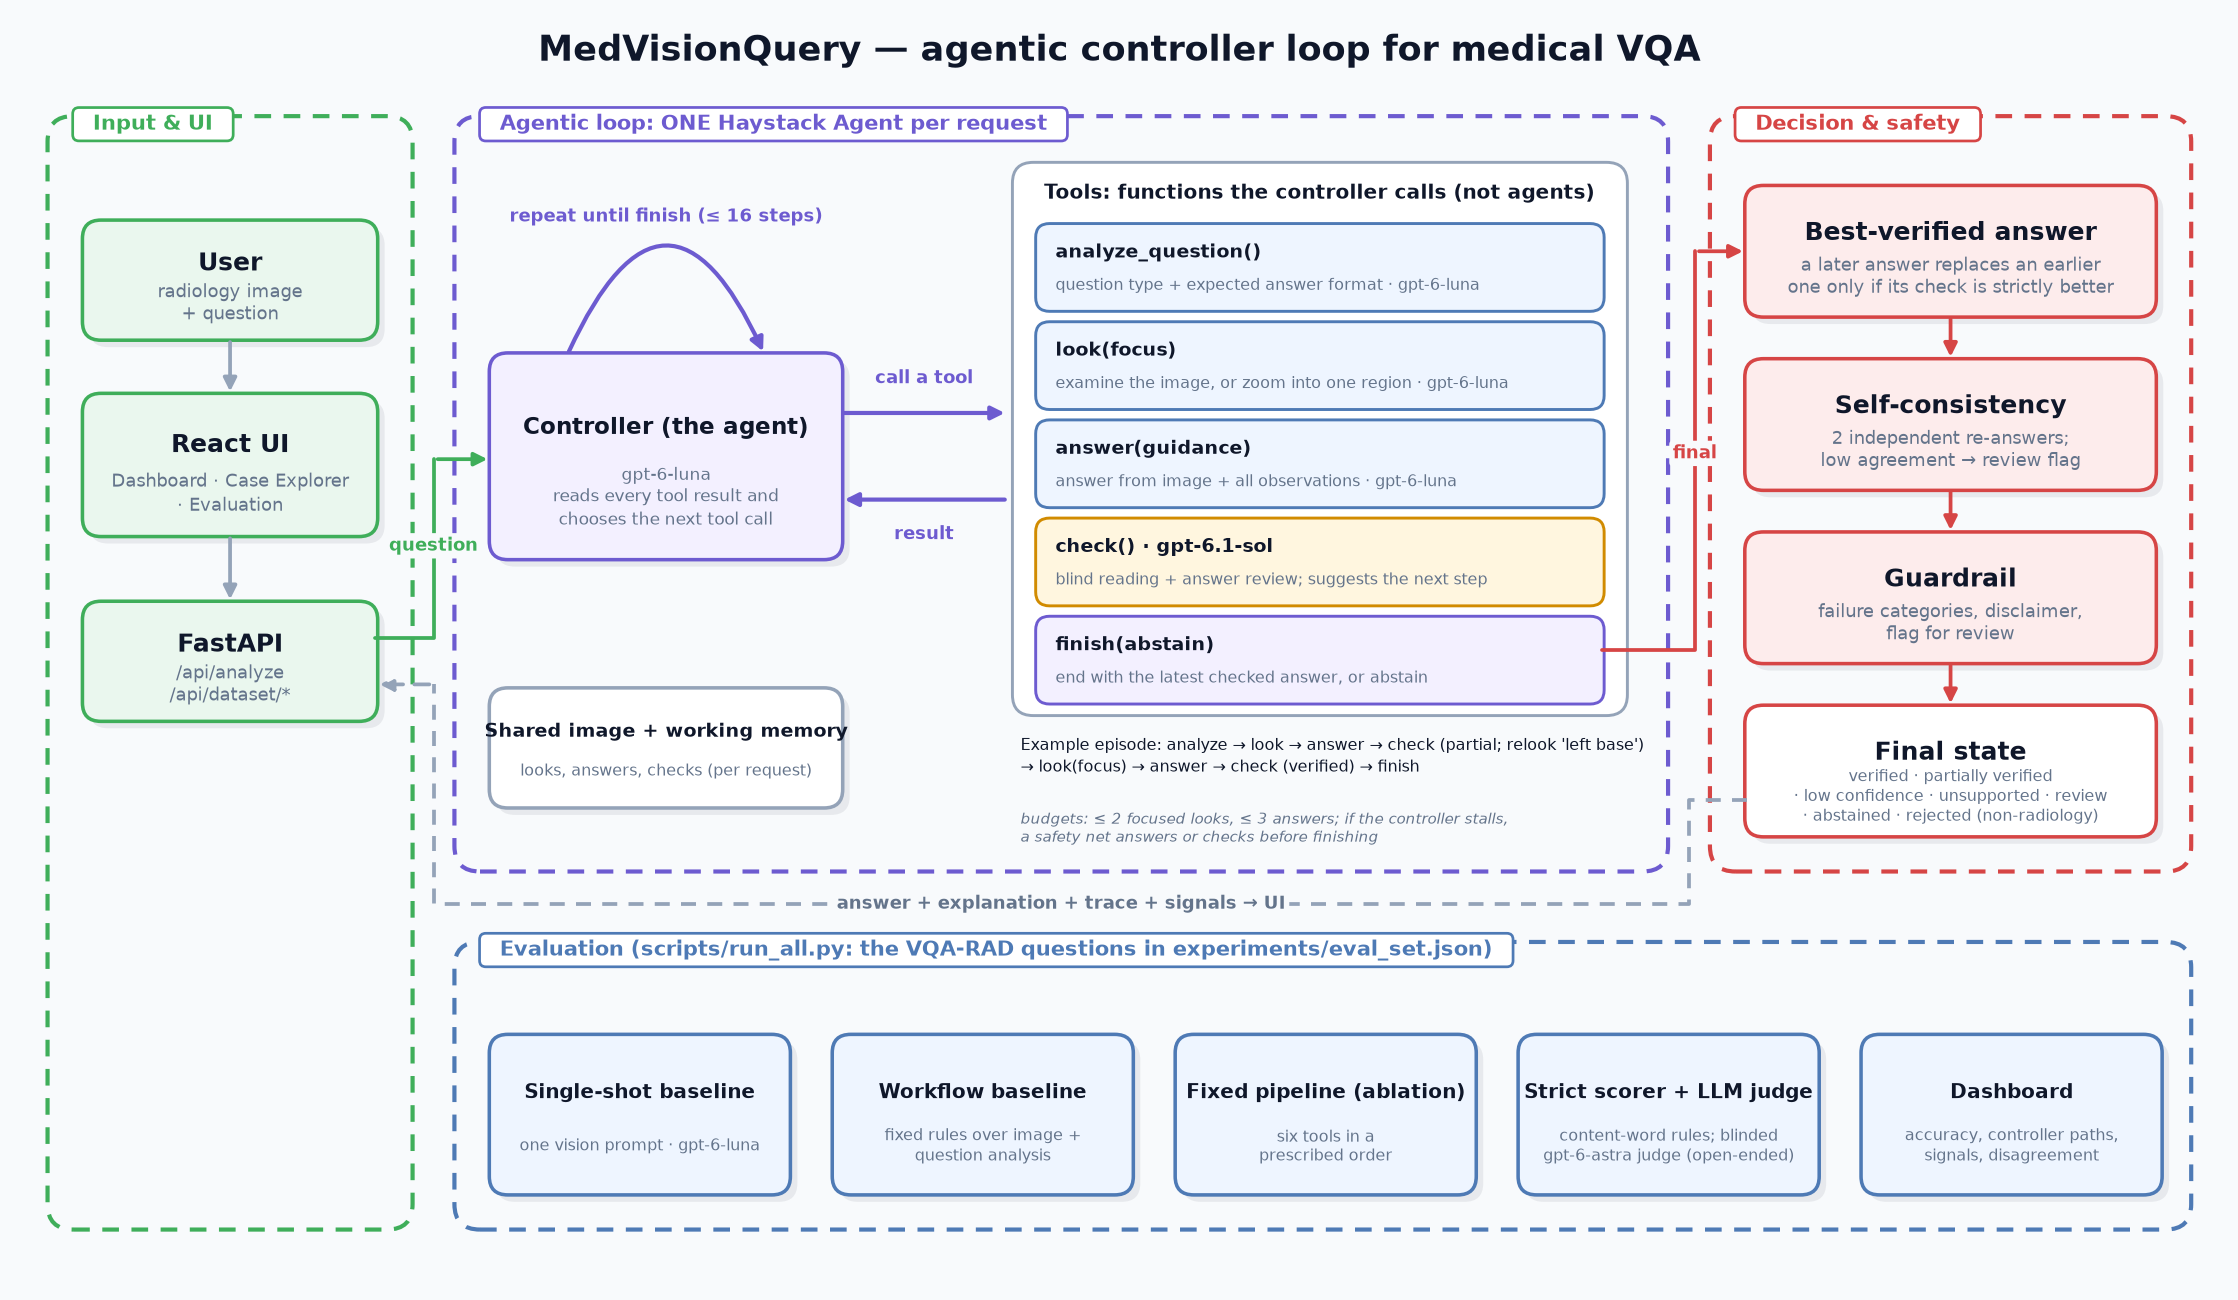
\includegraphics[width=\linewidth]{system_diagram.png}
  \caption{MedVisionQuery. One Haystack Agent (the controller) calls five tools in a loop, reading each result
  before choosing the next: question analysis, question-aware perception (\texttt{look}), answer synthesis,
  image-grounded verification (\texttt{check}) and \texttt{finish}. The tools are not agents; \texttt{check} only
  recommends a re-look, a revised answer, abstention or acceptance, and the controller decides. A decision-and-safety stage keeps the
  best-verified answer, measures self-consistency and applies guardrails.}
  \label{fig:arch}
\end{figure}

\paragraph{Controller loop.} A fresh Haystack \texttt{Agent} is created per request (Figure~\ref{fig:arch}). Its
five tools are bound to per-request working memory holding the image, the question analysis, and every look,
answer and check; the controller sees only short text results and chooses the next call. Unlike our earlier
fixed pipeline, the tool sequence depends on what verification finds: on the 200 evaluation cases the controller
finished directly in 141 cases, re-examined a region in 19, revised its answer in 29 and abstained in 11. Budgets
cap the loop at two focused re-looks, three answers and 16 steps, with a safety net that checks the latest answer
if the controller stalls.

\paragraph{Roles.} The \emph{controller} is the planner: it chooses every next step from the results so far.
The per-request \emph{working memory} (image, question analysis, looks, answers, checks) is the memory; the tools
read from and write to it.
\textbf{\texttt{analyze\_question}} (task understanding) classifies the question type and expected answer format.
\textbf{\texttt{look(focus)}} (perception) examines the image \emph{with the question in mind}; with a focus, it
re-examines a named region; the first look rejects non-radiology images.
\textbf{\texttt{answer(guidance)}} (executor) answers from the image plus all observations, applying the
verifier's guidance on revisions.
\textbf{\texttt{check}} (evaluator) verifies the answer against the image with five checks, returns a status
(verified, partially verified, low confidence, unsupported) and recommends \emph{accept}, \emph{relook} with a
focus, \emph{reanswer} with guidance, or \emph{abstain}.
\textbf{\texttt{finish(abstain)}} ends the episode and is refused while the latest answer is unchecked.

\paragraph{Model and tool choices.} All roles use OpenAI models, sized by need and configurable per role. The
controller and question analysis make simple decisions (\texttt{gpt-6-luna}, no/low reasoning effort); perception
and answering use \texttt{gpt-6-luna} with medium effort, and the answerer always sees the image: in a 20-case
pilot that alone raised accuracy from 50\% to 70\%. Verification uses a different, larger model
(\texttt{gpt-6.1-sol}) so that the answering model does not verify itself. Haystack's \texttt{Agent}/\texttt{Tool}
abstraction provides the tool-calling loop and exit conditions; keeping the image in per-request memory rather than
in the controller's context keeps the controller cheap. An earlier retrieval stage over SLAKE~\cite{liu2021slake} was
removed: it returned other patients' question--answer pairs, which contradicted yes/no and location answers and gave
no measurable benefit on perception-bound questions.

\paragraph{Baselines and ablation.} The \emph{single-shot baseline} sends the image and question in one prompt. The
\emph{workflow baseline} is a fixed chain---a question-agnostic image description, question analysis, then
hand-written rules per question type. The \emph{fixed-pipeline ablation} runs our original six stages (interpret,
analyse, filter, route, reason, verify, with retry) in a fixed order with the image given to the reasoner, isolating
what the controller's decisions add. A demo UI (Section~\ref{sec:ui}) exposes all systems.

% ============================================================================
\section{Multimodal Grounding}
% ============================================================================
The system uses two modalities, the radiology image and the text question, and they interact at every step that
determines the answer: the question (and any focus) steers what \texttt{look} examines; \texttt{answer} and
\texttt{check} receive the image directly alongside the text observations; only the controller works purely in
text. Our earlier design described the image once, \emph{without} the question, and passed only that text downstream;
in a 20-case pilot, giving the reasoner the image raised accuracy from 10/20 to 14/20, and typical text-only
failures were ``cannot be determined from the provided image description''. Because the verifier sees the image, its
``explanation grounded in evidence'' and ``no contradictions'' checks are genuine cross-modal agreement checks.

% ============================================================================
\section{Control and Failure Handling}
% ============================================================================
\textbf{Detection.} Image-grounded verification (five checks and a status), seven failure categories
(\emph{unsupported claim}, \emph{low confidence}, \emph{visual contradiction}, \emph{partially verified},
\emph{question--answer mismatch}, \emph{generation unstable}, \emph{parser failure}) and an eighth,
\emph{self-inconsistent}, from resampling.
\textbf{Recovery.} Instead of re-running the whole pipeline, the controller re-examines the region the verifier
names or revises the answer with the verifier's guidance. A later answer replaces an earlier one only if its check
is strictly better, because focused re-looks can over-read.
\textbf{Self-critique.} After finishing, the answerer is re-asked independently twice; low agreement adds a failure
category and flags the case for review.
\textbf{Fallback.} The controller may abstain (reported as an abstention, never coerced into ``no''); a guardrail
adds a disclaimer and a review flag for low-confidence, unsupported, high-severity or self-inconsistent cases;
non-radiology or unreadable images are rejected before any answer is produced.

% ============================================================================
\section{Evaluation}
% ============================================================================
\paragraph{Setup.} 200 VQA-RAD test questions drawn at random (seed 42; 111 close-ended, 89 open-ended); all four
systems run on the same cases with the same answering model. \emph{Strict scoring}: yes/no answers must start with
the correct word; binary terms must name the correct term and not its opposite; counts must match; open-ended answers
must contain every content word of the reference (aliases and plurals folded; $\geq$60\% for references longer than
three words), with left/right conflicts and denials counted wrong and embedding similarity~\cite{deka2022spubmed}
only as a strict fallback. Because strict scoring rejects correct paraphrases, a \emph{blinded LLM judge}
(\texttt{gpt-6.1-sol}, answers shuffled and anonymised) re-assesses strict-wrong open-ended answers; a 30-verdict
spot check agreed on 29/30 credit decisions. Paired comparisons use the exact McNemar test; 95\% intervals are about
$\pm$6.7 points. The baseline and agentic loop were re-run on 50 cases to measure stability. API cost of the
evaluation: \$4.08 (\$3.43 runs, \$0.54 repeats, \$0.11 judge). Actual wall-clock time: 40\,min for the
main run (four cases at a time), 35\,min for the 50 sequential repeats and 6\,min for the judge.

\begin{table}[t]
  \centering
  \caption{Accuracy (\%) on 200 random VQA-RAD test questions (same answering model for all systems). Open-ended accuracy is strict/judged. Time is per-case latency in seconds (mean/median), measured with four cases running concurrently; the whole 200-case run of all four systems took 40 minutes of wall-clock time. Cost is the mean API cost per case.}
  \label{tab:main}
  \small
  \begin{tabular}{lcccccc}
    \toprule
    System & Strict & Judged & Close (111) & Open (89) & Time (s) & Cost \\
    \midrule
    Single-shot baseline      & 63.5 & 70.0 & 76.6 & 47.2 / 61.8 & 4.4 / 3.6  & \$0.0002 \\
    Workflow baseline         & 28.0 & 31.0 & 42.3 & 10.1 / 16.9 & 9.0 / 8.7  & \$0.0005 \\
    \textbf{Agentic loop}     & \textbf{64.5} & \textbf{72.0} & 76.6 & 49.4 / 66.3 & 37.2 / 29.3 & \$0.0094 \\
    Fixed pipeline (ablation) & 57.0 & 61.5 & 68.5 & 42.7 / 52.8 & 38.1 / 29.4 & \$0.0070 \\
    \bottomrule
  \end{tabular}
\end{table}

\paragraph{Results.} Table~\ref{tab:main}. The agentic loop and the single prompt are statistically
indistinguishable (17 vs.\ 15 discordant cases, $p=0.86$; judged $p=0.61$). The controller's decisions clearly help
relative to the same models in a fixed order (26 vs.\ 11, $p=0.02$; judged 32 vs.\ 11, $p=0.002$), and both far
exceed the hand-designed workflow. Gains concentrate where the controller acts: on cases it re-examined it scored
47\% versus 37\% for the single prompt, and on revised cases 55\% versus 45\% (Table~\ref{tab:paths}).

\begin{table}[t]
  \centering
  \caption{Left: accuracy (strict, \%) by the path the controller took. Right: agentic accuracy by its own signals.}
  \label{tab:paths}
  \small
  \begin{tabular}{lcccc@{\hskip 18pt}lc}
    \toprule
    Path & $n$ & Agentic & Single & Pipeline & Signal & Agentic \\
    \midrule
    direct    & 141 & 74 & 72 & 67 & verified (169)            & 70 \\
    relook    & 19  & 47 & 37 & 37 & partially verified (25)   & 40 \\
    reanswer  & 29  & 55 & 45 & 31 & unsupported/low (6)       & 0  \\
    abstained & 11  & -- & 45 & 36 & consistency high (162)    & 72 \\
              &     &    &    &    & consistency med/low (27)  & 40--53 \\
    \bottomrule
  \end{tabular}
\end{table}

\paragraph{Failure case analysis.}
\emph{Self-consistency:} two independent re-answers per case; high consistency means 72\% accuracy, medium/low
40--53\%, so low consistency marks uncertainty rather than certain error.
\emph{Cross-modal agreement:} because the verifier sees the image, verification status is predictive: verified
answers are 70\% correct, unsupported or low-confidence answers 0\%.
\emph{Verifier model:} a larger model verifying a smaller one steers 59 of 200 episodes away from the direct path.
\emph{Disagreement:} the three systems disagree on 65\% of cases; when exactly one system is right, it is the agentic
loop 16 times, the single prompt 12 and the workflow 7.
\emph{Stability:} on 50 repeated cases, 12\% of single-prompt answers flipped between right and wrong, versus 2\% for
the agentic loop.
Four patterns dominate the errors: (i) a shared perception blind spot, where looker and verifier misread the image the
same way (e.g.\ bowel gas read as free air after two focused re-looks); (ii) over-reading on re-looks, limited by
keeping the best-verified answer; (iii) benchmark items whose question does not match the image, which every system
fails; and (iv) workflow rigidity, where fixed rules answer ``Brain'' or ``X-ray'' when a specific finding is needed.

% ============================================================================
\section{User Interface}\label{sec:ui}
% ============================================================================
A React frontend exposes three views: \textbf{Dashboard} (upload an image, compare the agentic loop with both
baselines, inspect the trace, verification checks and failure categories), \textbf{Case Explorer} (browse the 200
evaluation cases with full agent traces) and \textbf{Evaluation} (strict and judged accuracy for all four systems,
accuracy by question type and by controller path, disagreement and a per-case table).

% ============================================================================
\section{Reflection}
% ============================================================================
\paragraph{When agentic behaviour is beneficial.} Not for raw accuracy on this benchmark: a strong single prompt on
the same model is as accurate. The agentic system pays off when answers must be \emph{trustworthy}: its
verification and consistency signals identify likely errors, it abstains on cases where the single prompt is wrong
more often than right, it recovers on hard cases by re-examining specific regions, its answers are far more stable
across runs, and every decision is auditable. Against a fixed multi-stage pipeline with identical models, letting a
controller decide is clearly better---the benefit comes from \emph{adaptive control}, not from decomposition alone.

\paragraph{Limitations.} About 41$\times$ the cost and 8$\times$ the latency of a single prompt for equal accuracy.
The verifier shares the perception weaknesses of vision models, so agreement is not correctness. Two hundred cases
give $\pm$6.7-point intervals and noisy per-type estimates; the LLM judge is an upper bound, spot-checked but not
human-annotated. A retrieval stage did not help perception-bound questions and was removed; retrieval may still
help questions that need knowledge not visible in the image, which VQA-RAD rarely contains.

% ============================================================================
\begin{thebibliography}{15}
\small

\bibitem{lin2023survey}
Lin, Z., Zhang, D., Tao, Q., Shi, D., Haffari, G., Wu, Q., He, M., \& Ge, Z. (2023). Medical visual question
answering: A survey. \emph{Artificial Intelligence in Medicine}, 143, 102611.

\bibitem{liu2023q2a}
Liu, Y., Wang, Z., Xu, D., \& Zhou, L. (2023). Q2ATransformer: Improving medical VQA via an answer querying decoder.
In \emph{Information Processing in Medical Imaging -- IPMI 2023}, Lecture Notes in Computer Science, vol.~13939,
pp.~445--456. Springer.

\bibitem{liu2023conditional}
Liu, B., Zhan, L.M., Xu, L., \& Wu, X.M. (2023). Medical visual question answering via conditional reasoning and
contrastive learning. \emph{IEEE Transactions on Medical Imaging}, 42(5), 1532--1545.

\bibitem{qiu2025chain}
Qiu, C., Huang, K., Xie, Z., Liu, M., Gu, J., \& Zong, X. (2025). Explainable medical visual question answering via
chain of evidence. \emph{Knowledge-Based Systems}. doi:10.1016/j.knosys.2025.113672.

\bibitem{syed2025medvctp}
Syed, A., et al. (2025). MedVCTP: Improving accuracy and explainability in medical visual reasoning. In
\emph{NeurIPS 2025 Workshop on Human-AI Coevolution (HAIC)}.

\bibitem{benabacha2019vqamed}
Ben Abacha, A., Hasan, S.A., Datla, V.V., Liu, J., Demner-Fushman, D., \& M\"uller, H. (2019). VQA-Med: Overview of
the medical visual question answering task at ImageCLEF 2019. \emph{Working Notes of CLEF 2019}.

\bibitem{nguyen2019mevf}
Nguyen, B.D., Do, T.T., Nguyen, B.X., Do, T., Tjiputra, E., \& Tran, Q.D. (2019). Overcoming data limitation in
medical visual question answering. In \emph{MICCAI 2019}, Lecture Notes in Computer Science, pp.~522--530. Springer.

\bibitem{zhang2023pmcvqa}
Zhang, X., Wu, C., Zhao, Z., Lin, W., Zhang, Y., Wang, Y., \& Xie, W. (2023). PMC-VQA: Visual instruction tuning for
medical visual question answering. \emph{arXiv preprint arXiv:2305.10415}.

\bibitem{bazi2023}
Bazi, Y., Al Rahhal, M.M., Bashmal, L., \& Zuair, M. (2023). Vision--language model for visual question answering in
medical imagery. \emph{Bioengineering}, 10(3), 380.

\bibitem{li2023llavamed}
Li, C., Wong, C., Zhang, S., Usuyama, N., Liu, H., Yang, J., Naumann, T., Poon, H., \& Gao, J. (2023). LLaVA-Med:
Training a large language-and-vision assistant for biomedicine in one day. In \emph{Advances in Neural Information
Processing Systems (NeurIPS 2023), Datasets and Benchmarks Track}.

\bibitem{wu2025radfm}
Wu, C., Zhang, X., Zhang, Y., Hui, H., Wang, Y., \& Xie, W. (2025). Towards generalist foundation model for radiology
by leveraging web-scale 2D\&3D medical data. \emph{Nature Communications}, 16, 7866.

\bibitem{chen2025rllava}
Chen, X., Lai, Z., Ruan, K., Chen, S., Liu, J., \& Liu, Z. (2025). R-LLaVA: Improving Med-VQA understanding through
visual region of interest. In \emph{ICLR 2025 Workshop on Human-AI Coevolution (HAIC)}.
\url{https://arxiv.org/abs/2410.20327}.

\bibitem{lau2018vqarad}
Lau, J.J., Gayen, S., Ben Abacha, A., \& Demner-Fushman, D. (2018). A dataset of clinically generated visual questions
and answers about radiology images. \emph{Scientific Data}, 5:180251.

\bibitem{deka2022spubmed}
Deka, P., Jurek-Loughrey, A., \& Deepak, P. (2022). Improved methods to aid unsupervised evidence-based fact checking
for online health news. \emph{Journal of Data Intelligence}, 3(4), 474--504.
\url{https://huggingface.co/pritamdeka/S-PubMedBert-MS-MARCO}.

\bibitem{liu2021slake}
Liu, B., Zhan, L.M., Xu, L., Ma, L., Yang, Y., \& Wu, X.M. (2021). SLAKE: A semantically-labeled knowledge-enhanced
dataset for medical visual question answering. In \emph{Proceedings of the IEEE 18th International Symposium on
Biomedical Imaging (ISBI 2021)}, pp.~1650--1654. IEEE.

\end{thebibliography}

\end{document}
